\normaltrue
\correctiontrue

%\UPSTIidClasse{11} % 11 sup, 12 spé
%\newcommand{\UPSTIidClasse}{11}


\exer{Mouvement TT -- $\star$ \label{C1:05:03:PFD}}
\setcounter{question}{0}\UPSTIcompetence[2]{B2-14}
\UPSTIcompetence[2]{C1-05}
\index{Compétence B2-14}
\index{Compétence C1-05}
\index{Principe fondamental de la dynamique}
\index{PFD}
\index{Mécanisme à 2 translations}
\ifcorrection
\else
\marginnote{\textbf{Pas de corrigé pour cet exercice.}}
\fi

\ifprof
\else
Soit le mécanisme suivant. On note $\vect{AB}=\lambda(t)\vect{i_0}$ et $\vect{BC}=\mu(t)\vect{j_0}$.
$G_1 = B$ désigne le centre d'inertie de \textbf{1},et $m_1$ sa masse. %et $\inertie{G_1}{1}=\matinertie{A_1}{B_1}{C_1}{0}{0}{0}{\bas{1}}$; 
$G_2 = C$ désigne le centre d'inertie de \textbf{2} et  $m_2$ sa masse. % et $\inertie{G_2}{2}=\matinertie{A_2}{B_2}{C_2}{0}{0}{0}{\bas{2}}$.

 Un vérin électrique positionné entre \textbf{0} et \textbf{1} permet d'actionner le solide \textbf{1}.
 Un vérin électrique positionné entre \textbf{1} et \textbf{2} permet d'actionner le solide \textbf{2}.

L'accélération de la pesanteur est donnée par $\vect{g}=-g\vect{j_0}$.

\begin{center}
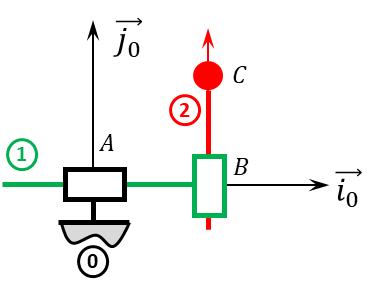
\includegraphics[width=.6\linewidth]{03_TT_01}
\end{center}
\fi

\question{Réaliser le graphe d'analyse en faisant apparaître l'ensemble des actions mécaniques.}
\ifprof
\begin{center}
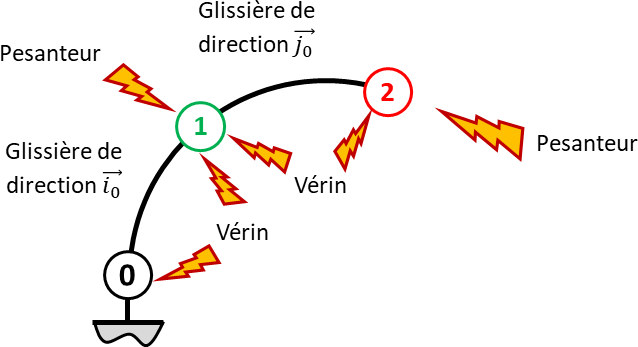
\includegraphics[width=.6\linewidth]{03_TT_01_cor}
\end{center}
\else
\fi

\question{Proposer une démarche permettant de déterminer les loi de mouvement de \textbf{1} et de \textbf{2} par rapport à $\rep{0}$.}
\ifprof
C'est une chaîne ouverte. On isole l'extrémité et on applique le théorème correspondant la mobilité : 
\begin{itemize}
\item on isole \textbf{2} et on réalise le théorème de la résultante dynamique en projection sur $\vj{0}$;
\item on isole \textbf{1+2} et on réalise le théorème de la résultante dynamique en projection sur $\vi{0}$.
\end{itemize}
\else
\fi


\ifprof
\else
\begin{flushright}
\footnotesize{Corrigé  voir \ref{C1:05:03:PFD}.}
\end{flushright}%
\fi